
% \titlegraphic{\hfill\includegraphics[height=1.5cm]{logo.pdf}}

\documentclass[xcolor=pdftex,dvipsnames,table,numbers,hyperref={pdfpagelabels=false},compress]{beamer}
%\usepackage{requiredPackage}
\usepackage{amsmath}
\usepackage{graphicx}
\usepackage{amsfonts}
\usepackage{amssymb}

\usepackage{tabularx}
\usepackage{epstopdf}
\usepackage{overpic}
\usepackage{url}
\usepackage{calrsfs}
\usepackage{mathrsfs}
\usepackage{epsfig}
\usepackage{cancel}
\usepackage{changepage}

\usepackage{tikz}
\usepackage[customcolors]{hf-tikz} 

\usepackage{lmodern}
%\usepackage{mystyle}
\usepackage{subfig}
\usepackage{pifont}
\usepackage{tabu}
\usepackage{xcolor}
\usepackage{algorithm}
\usepackage{algpseudocode}
%\usepackage{enumitem}
\usepackage{remreset}
\usepackage{etoolbox}
\usepackage{comment} % end and begin comment
%\usepackage{dtklogos} 
\usepackage{listings}
\lstset{breaklines=true} 

\newcommand{\gline}{\textcolor{gray}{\hline}}
\newcommand{\cmark}{\ding{51}}%
\newcommand{\xmark}{\ding{55}}%
\newcommand{\gcheck}{\textcolor{blue}{\Large \cmark}}
\newcommand{\rcross}{\textcolor{red}{\Large \xmark}}
\newcommand{\tkt}{\tilde{K}_\theta}
\newcommand{\kt}{K_\theta}
\newcommand{\ind}{\overset{ind}{\sim}}
\newcommand{\plim}{\overset{p}{\rightarrow}}
\newcommand{\cx}{\frac {X'X}n}
\newcommand{\cz}{\frac {Z'Z}n}
\newcommand{\ccz}{\frac {Z'Z}n - \Sigma_A}
\newcommand{\czy}{\frac {Z'y}n}
\newcommand{\cyz}{\frac {y'Z}n}
\newcommand{\cxy}{\frac {X'y}n}
\newcommand{\cyx}{\frac {y'X}n}
\newcommand{\myitem}{\vskip3mm \item}

\newcommand{\calS}{{\cal S}}
\newcommand{\calA}{{\cal A}}
\newcommand{\calK}{{\cal K}}
\newcommand{\calX}{{\cal X}}
\newcommand{\calD}{{\cal D}}
\newcommand{\calG}{{\cal G}}
\newcommand{\calT}{{\cal T}}
\newcommand{\calU}{{\cal U}}
\newcommand{\calR}{{\cal R}}
\newcommand{\tp}{\tilde{p}}
\newcommand{\tildebC}{\tilde{\bC}}
\newcommand{\calL}{{\cal L}}

\newcommand{\blam}{ \mbox{\boldmath $ \lambda $} }
\newcommand{\bet}{ \mbox{\boldmath $ \eta $} }
\newcommand{\bome}{ \mbox{\boldmath $ \omega $} }
\newcommand{\bbet}{ \mbox{\boldmath $ \beta $} }
\newcommand{\bbeta}{ \mbox{\boldmath $ \beta $} }
\newcommand{\balph}{ \mbox{\boldmath $ \alpha $} }
\newcommand{\balpha}{ \mbox{\boldmath $ \alpha $} }
\newcommand{\bphi}{ \mbox{\boldmath $\phi$}}
\newcommand{\bzeta}{ \mbox{\boldmath $\zeta$}}
\newcommand{\bkap}{ \mbox{\boldmath $\kappa$}}
\newcommand{\bkappa}{ \mbox{\boldmath $\kappa$}}
\newcommand{\beps}{ \mbox{\boldmath $\epsilon$}}
\newcommand{\bepsilon}{ \mbox{\boldmath $\epsilon$}}
\newcommand{\bthet}{ \mbox{\boldmath $ \theta $} }
\newcommand{\btheta}{ \mbox{\boldmath $ \theta $} }
\newcommand{\blambda}{ \mbox{\boldmath $ \lambda $} }
\newcommand{\bnu}{ \mbox{\boldmath $\nu$} }
\newcommand{\bmu}{ \mbox{\boldmath $\mu$} }
\newcommand{\bGam}{ \mbox{\boldmath $\Gamma$} }
\newcommand{\bSig}{ \mbox{\boldmath $\Sigma$} }
\newcommand{\bSigma}{ \mbox{\boldmath $\Sigma$} }
\newcommand{\bPhi}{ \mbox{\boldmath $\Phi$} }
\newcommand{\bThet}{ \mbox{\boldmath $\Theta$} }
\newcommand{\bTheta}{ \mbox{\boldmath $\Theta$} }
\newcommand{\bDel}{ \mbox{\boldmath $\Delta$} }
\newcommand{\bDelta}{ \mbox{\boldmath $\Delta$} }
\newcommand{\bnabla}{ \mbox{\boldmath $\nabla$} }
\newcommand{\bLam}{ \mbox{\boldmath $\Lambda$} }
\newcommand{\bLambda}{ \mbox{\boldmath $\Lambda$} }
\newcommand{\bgam}{ \mbox{\boldmath $\gamma$} }
\newcommand{\bgamma}{ \mbox{\boldmath $\gamma$} }
\newcommand{\brho}{ \mbox{\boldmath $\rho$} }
\newcommand{\bdel}{ \mbox{\boldmath $\delta$} }
\newcommand{\bdelta}{ \mbox{\boldmath $\delta$} }
\newcommand{\sis}{\sigma^2}
\newcommand{\bOmega}{\mbox{\boldmath $\Omega$} }
\newcommand{\bPsi}{ {\boldsymbol \Psi} }
\newcommand{\btkt}{\boldsymbol{\tilde{K}}_\theta}
\newcommand{\pg}{P{\'o}lya-Gamma }

\newcommand{\bzero}{\textbf{0}}
\newcommand{\bones}{\textbf{1}}
\newcommand{\ba}{\textbf{a}}
\newcommand{\bb}{\textbf{b}}
\newcommand{\bB}{\textbf{B}}
%\newcommand{\bA}{\textbf{A}}
\newcommand{\bc}{\textbf{c}}
\newcommand{\bC}{\textbf{C}}
\newcommand{\bA}{\textbf{A}}
\newcommand{\bd}{\textbf{d}}
\newcommand{\bD}{\textbf{D}}
\newcommand{\be}{\textbf{e}}
\newcommand{\bE}{\textbf{E}}
\newcommand{\bk}{\textbf{k}}
\newcommand{\bK}{\textbf{K}}
\newcommand{\bh}{\textbf{h}}
\newcommand{\bs}{\textbf{s}}
\newcommand{\bS}{\textbf{S}}
\newcommand{\bH}{\textbf{H}}
\newcommand{\bI}{\textbf{I}}
\newcommand{\bt}{\textbf{t}}
\newcommand{\bu}{\textbf{u}}
\newcommand{\bv}{\textbf{v}}
\newcommand{\bw}{\textbf{w}}
\newcommand{\bW}{\textbf{W}}
\newcommand{\bx}{\textbf{x}}
\newcommand{\bX}{\textbf{X}}
\newcommand{\by}{\textbf{y}}
\newcommand{\bY}{\textbf{Y}}
\newcommand{\bz}{\textbf{z}}
\newcommand{\bZ}{\textbf{Z}}
\newcommand{\bL}{\textbf{L}}
\newcommand{\br}{\textbf{r}}
\newcommand{\bR}{\textbf{R}}
\newcommand{\bm}{\textbf{m}}
\newcommand{\bM}{\textbf{M}}
\newcommand{\given}{\,|\,}
\newcommand{\T}{\top}
\newcommand{\bV}{\textbf{V}}
\newcommand{\bJ}{\textbf{J}}
\newcommand{\blue}[1]{{\color{RoyalBlue!90} #1}}
\newcommand{\red}[1]{{\color{Red} #1}}
\newcommand{\green}[1]{{\color{Green} #1}}
\newcommand{\orange}[1]{{\color{Orange} #1}}
\newcommand{\titl}[1]{{\begin{large}\begin{center}#1\end{center}\end{large}}}

\newcommand{\tildea}{\tilde{a}}
\newcommand{\tildeba}{\tilde{\ba}}
\newcommand{\tildebv}{\tilde{\bv}}
\newcommand{\tildev}{\tilde{v}}
\newcommand{\tildeA}{\tilde{A}}
\newcommand{\tildeC}{\tilde{C}}
\newcommand{\tildeK}{\tilde{K}}
\newcommand{\tildew}{\tilde{w}}
\newcommand{\tildeu}{\tilde{u}}
\newcommand{\tildebw}{\tilde{\bw}}
\newcommand{\tildeeps}{\tilde{\epsilon}}
\newcommand{\tildebeps}{\tilde{\bepsilon}}
\newcommand{\eps}{\epsilon}
\newcommand{\sigs}{\sigma^2}
\newcommand{\taus}{\tau^2}
\newcommand{\iid}{\stackrel{\mathrm{iid}}{\sim}}

%\newcommand{\calS}{{\cal S}}
\newcommand{\calC}{{\cal C}}

%\documentclass[10pt]{beamer}

\usetheme{metropolis}
\usepackage{appendixnumberbeamer}

\usepackage{booktabs}
\usepackage[scale=2]{ccicons}

\usepackage{pgfplots}
\usepgfplotslibrary{dateplot}

\usepackage{xspace}
\newcommand{\themename}{\textbf{\textsc{metropolis}}\xspace}

\makeatletter
\@addtoreset{subfigure}{framenumber}% subfigure counter resets every frame
\makeatother

\makeatletter
\@addtoreset{figure}{framenumber}% subfigure counter resets every frame
\makeatother

\setbeamertemplate{caption}{\raggedright\insertcaption\par}
\captionsetup[subfigure]{labelformat=empty}


\title[]{Introduction to Geostatistics}
\author{Andrew Finley$^1$ \& Jeffrey Doser$^2$}
	
\institute{
\begin{tiny}$^1$Department of Forestry, Michigan State University.\\
$^2$Department of Integrative Biology, Michigan State University.\end{tiny}
}

\date{May 15, 2023}


\begin{document}

\maketitle

\begin{frame}[plain]
\begin{itemize}
\item Course materials available at \href{tba}{tba}
\end{itemize}
\end{frame}


%\section{Introduction}
\begin{frame}{What is spatial data?}
	\begin{itemize}
		\item Any data with some geographical information
			\pause\myitem {Common sources of spatial data: climatology, forestry, ecology, environmental health, disease epidemiology, real estate marketing etc %\pause
			\begin{itemize}%\setlength{\itemsep}{0.3cm}
				\item have many important predictors and response variables %\pause
				\item are often presented as maps %\pause
				%\item and/or as data streaming in over time %\pause
			\end{itemize}}
			\pause\myitem Other examples where spatial need not refer to space on earth:
			\begin{itemize}
				\item Neuroimaging (data for each voxel in the brain)
				\item Genetics (position along a chromosome)
			\end{itemize}
	\end{itemize}
\end{frame}

\begin{frame}{Point-referenced spatial data}
	\begin{itemize}
				\item Each observation  is associated with a location (point) 
				\item Data represents a sample from a continuous spatial domain
				\item Also referred to as \alert {geocoded} or \alert {geostatistical} data
			\end{itemize}

		\begin{figure}
			\begin{center}
				\vskip -5mm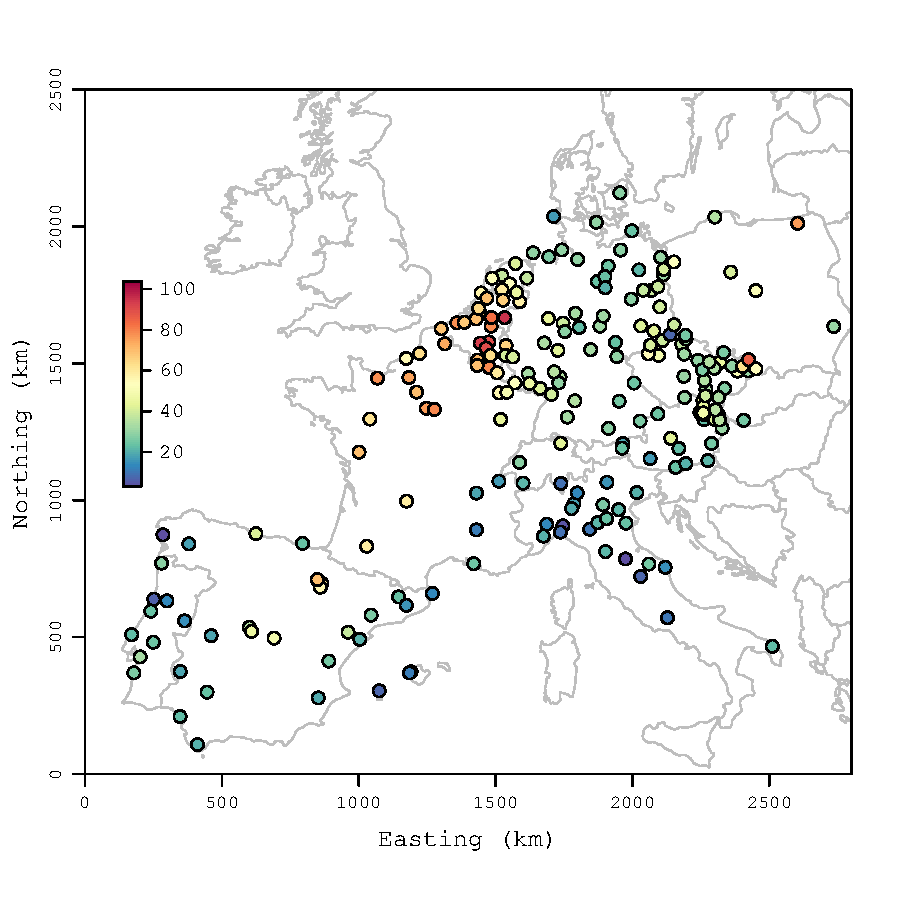
\includegraphics[width=5cm]{../figures/march-obs.pdf}
				\caption{Pollutant levels in Europe in March, 2009}
			\end{center}
		\end{figure}
\end{frame}

\begin{frame}{Point level modeling}
	\begin{itemize}
		\item \alert{Point-level modeling} refers to modeling of point-referenced data collected at locations referenced by \red{coordinates} (e.g., lat-long, Easting-Northing). %\pause
		
		\item Data from a spatial process $\{Y(s): s \in D\}$, $D$ is a subset in
		Euclidean space. %\pause
		
		\item \blue{Example:} $Y(s)$ is a \red{pollutant level} at site $s$ %\pause
		
		\item \red{Conceptually:} Pollutant level exists at all possible sites %\pause
		
		\item \blue{Practically:} Data will be a partial realization of a spatial process -- observed at $\{s_1,\ldots,s_n\}$ %\pause
		
		\item \red{Statistical objectives:} \blue{Inference} about the process $Y(s)$; \blue{predict} at new locations.
		
		\item \red{Remarkable:} Can learn about entire $Y(s)$ surface.  The \blue{key:} Structured dependence
	\end{itemize}
\end{frame}

%\section{Exploratory data analysis (EDA) for point-referenced data}
\begin{frame}{Exploratory data analysis (EDA): Plotting the data}
	\begin{itemize}
		\item A typical setup: Data observed at $n$ locations $\{s_1,\ldots,s_n\}$
		\item At each $s_i$ we observe the response $y(s_i)$ and a $p\times 1$ vector of covariates $x(s_i)'$
		\item \alert{Surface plots} of the data often helps to understand spatial patterns
	\end{itemize}
	\vskip-7mm\begin{figure}
	\subfloat[$y(s)$]{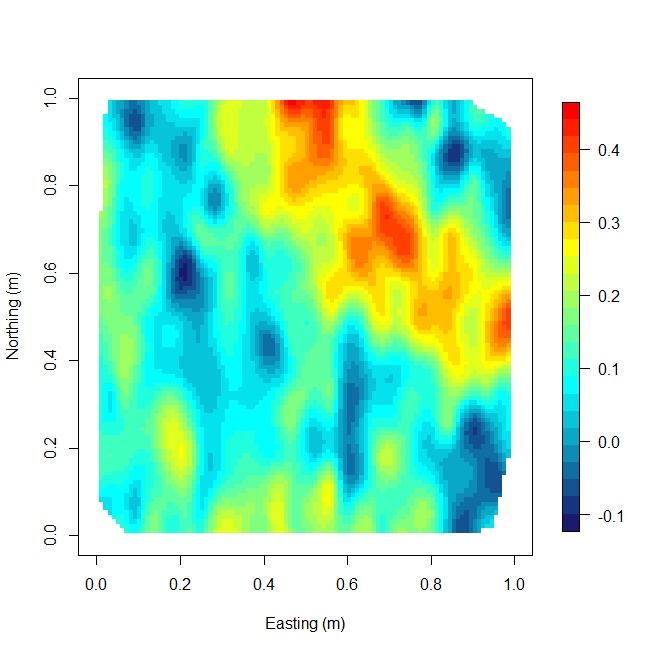
\includegraphics[scale=0.15,trim={0 5mm 0 5mm},clip]{../figures/data1_y.png}}
	\subfloat[$x(s)$]{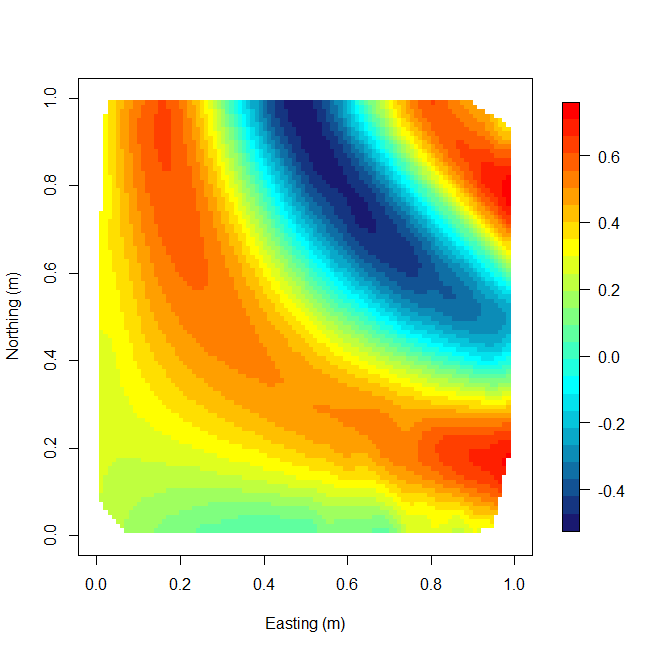
\includegraphics[scale=0.15,trim={0 5mm 0 5mm},clip]{../figures/data1_x.png}}\\
	\caption{Response and covariate surface plots for Dataset 1}
\end{figure}
\end{frame}

\begin{frame}{What's so special about spatial?}
	\begin{itemize}
		\item Linear regression model: $y(s_i)=x(s_i)'\beta + \eps(s_i)$
		\item $\eps(s_i)$ are iid $N(0,\tau^2)$ errors 
		\item $y=(y(s_1),y(s_2),\ldots,y(s_n))'$;  $X=(x(s_1)',x(s_2)',\ldots,x(s_n)')'$
		\item \blue{Inference:} $\hat\beta = (X'X)^{-1}X'Y \sim N(\beta, \tau^2 (X'X)^{-1})$
		\item \blue{Prediction} at new location $s_0$: $\widehat{y(s_0)} = x(s_0)'\hat\beta$
		\item Although the data is spatial, this is an \red{ordinary linear regression} model
		%\item Does this always suffice or we need any thing specialized method for such data?
	\end{itemize}
\end{frame}

\begin{frame}{Residual plots}
	\begin{itemize}
		\item Surface plots of the residuals ($y(s) - \widehat{y(s)}$) help to identify any spatial patterns left unexplained by the covariates 
	\end{itemize}
	\begin{figure}
		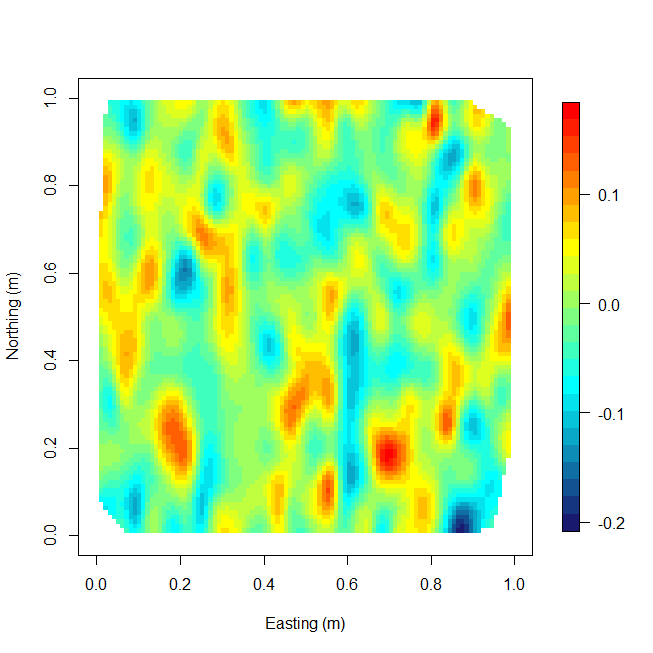
\includegraphics[scale=0.15,trim={2mm 5mm 2mm  5mm},clip]{../figures/data1_res.png}
		\caption{Residual plot for Dataset 1 after linear regression on $x(s)$}
	\end{figure}
	\pause
	\vskip -5mm \begin{itemize}
		\item No evident spatial pattern in plot of the residuals
		\item The covariate $x(s)$ seem to explain all spatial variation in $y(s)$
		\item \red{Does a non-spatial regression model always suffice?}
	\end{itemize}
\end{frame}

\begin{frame}{Western Experimental Forestry (WEF) data}
\begin{itemize}
	\item Data consist of a census of all trees in a 10 ha. stand in Oregon
	\item Response of interest: Diameter at breast height (DBH) 
	\item Covariate: Tree species (Categorical variable)
\end{itemize}

\begin{figure} 
	\begin{center}
		\vskip -8mm \subfloat[DBH]{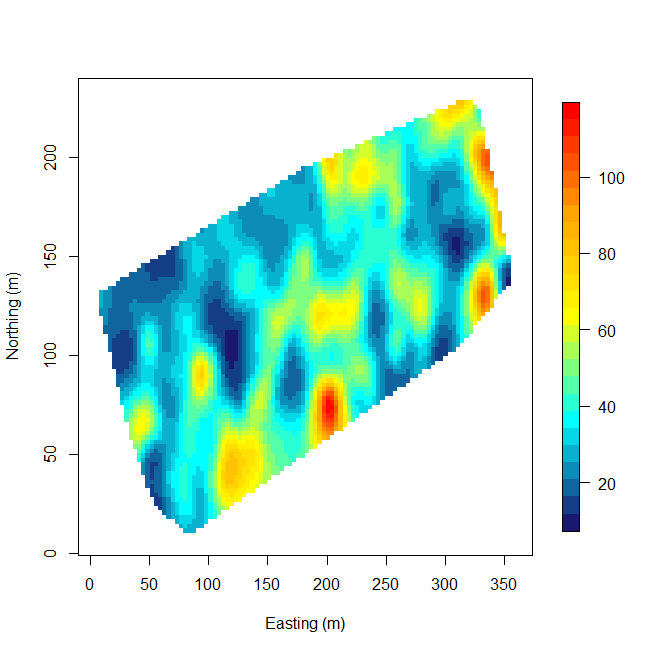
\includegraphics[scale=0.15]{../figures/wef_dbh_surf.png}}
		\subfloat[Species]{ 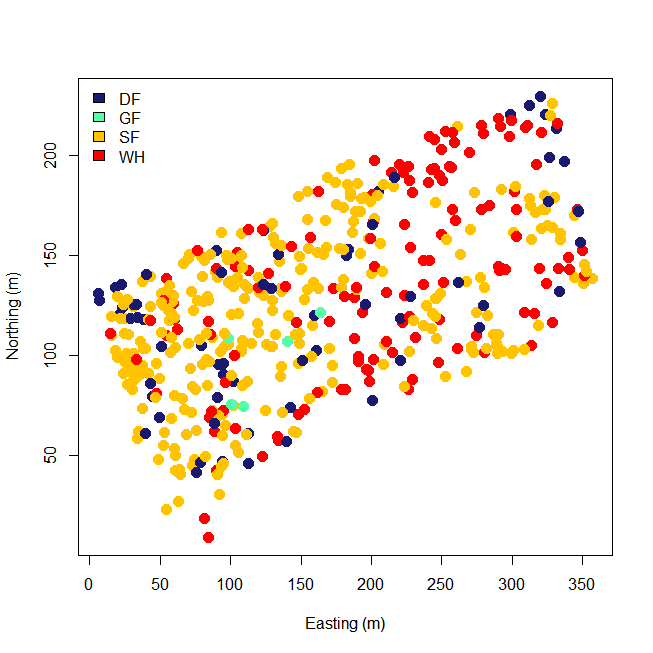
\includegraphics[scale=0.15]{../figures/wef_species.png}}
		\subfloat[Residuals]{ 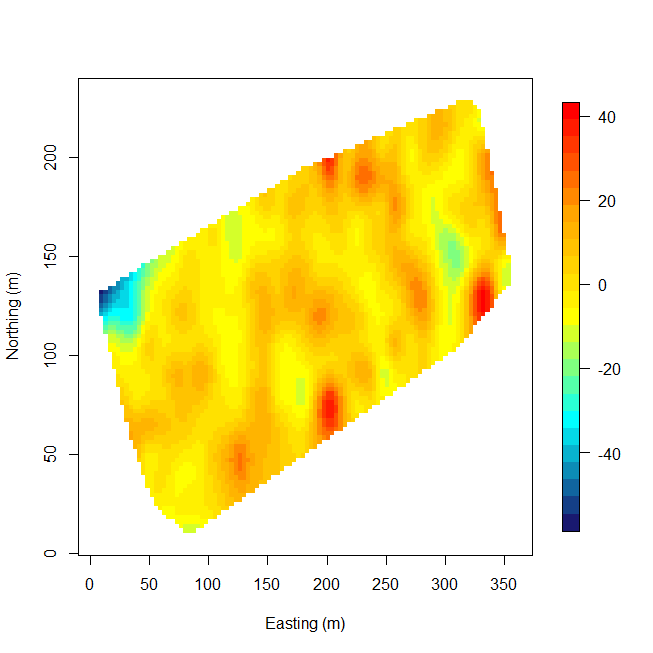
\includegraphics[scale=0.15]{../figures/wef_res.png}}
	\end{center}
\end{figure}
\pause
\begin{itemize}
	\item \red{Local spatial patterns} in the residual plot
	\item Simple regression on species seems to be \red{not sufficient}
\end{itemize}
\end{frame}



\begin{frame}{More EDA}
	\begin{itemize}
		\item Besides eyeballing residual surfaces, how to do more formal EDA to identify spatial pattern ?
	\end{itemize}
	\pause
	\metroset{block=fill}
      \begin{exampleblock}{First law of geography}
{\em "Everything is related to everything else, but \red{near things are more related} than distant things."} -- Waldo Tobler
		\end{exampleblock}
	
	\pause
	\begin{itemize}
		%\item The residual surface seems continuous 
		%\item If a spatial surface $Y(s)$ is continuous then $(Y(s+h)-Y(s))^2 \rightarrow 0$ as $||h|| \rightarrow 0$
		\item In general $(Y(s+h)-Y(s))^2$ roughly increasing with $||h||$ will imply a spatial correlation
		\item Can this be formalized to identify spatial pattern?
	\end{itemize}
\end{frame}

\begin{frame}{Empirical semivariogram}
	\begin{itemize}
		\item \blue{Binning:} Make intervals $I_1=(0,m_1)$,
		$I_2=(m_1,m_2)$, and so forth, up to $I_K=(m_{K-1},m_K)$.
		Representing each interval by its midpoint $t_k$, we
		define:
		\[
		N(t_k) = \{(s_i,s_j): \|s_i - s_j\| \in I_k \},
		k=1,\ldots,K.
		\]
		\item \alert{Empirical semivariogram:}
		\[
		\gamma(t_k) = \frac{1}{2|N(t_k)|}\sum_{s_i,s_j \in
			N(t_k)}(Y(s_i)-Y(s_j))^2
		\]
		%\item Semivariogram = $0.5\times$Variogram
		\item For spatial data, the $\gamma(t_k)$ is expected to roughly increase with $t_k$
		\item A flat semivariogram would suggest little spatial variation
	\end{itemize}
\end{frame}

\begin{frame}{Empirical variogram: Data 1}
	\begin{figure}
		\subfloat[y]{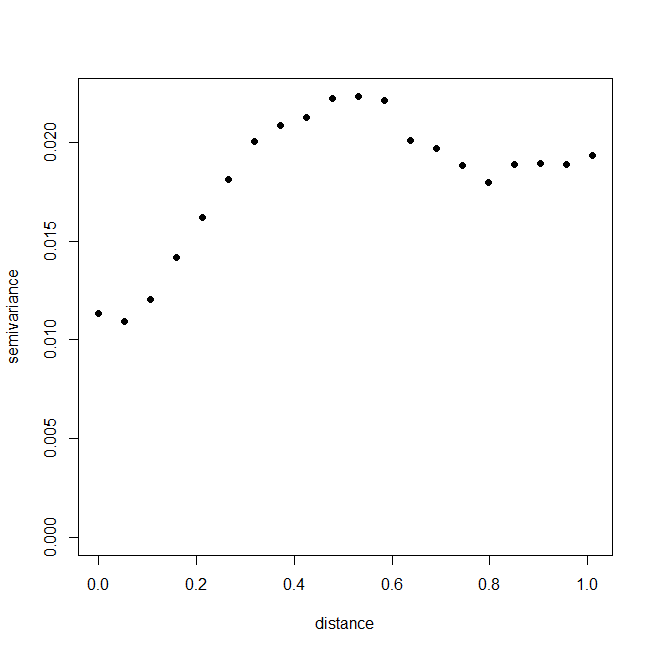
\includegraphics[scale=0.2,trim={2mm 5mm 2mm  5mm},clip]{../figures/data1_vario.png}}
		\subfloat[residuals]{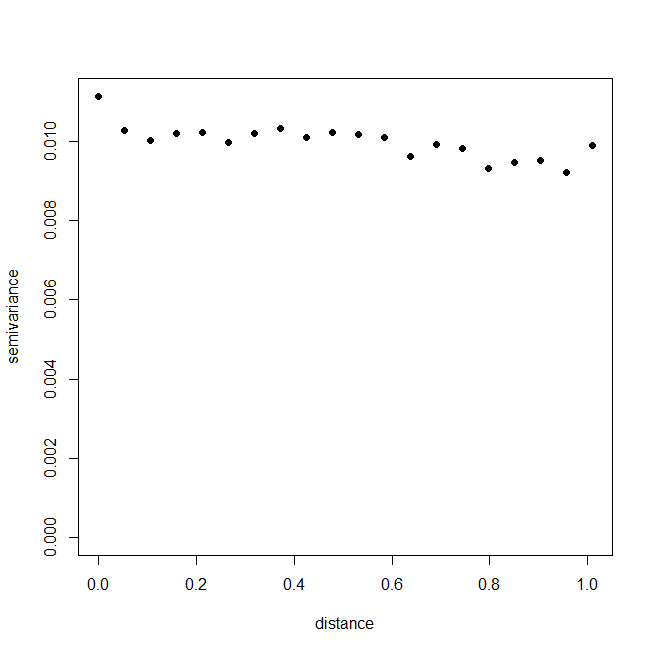
\includegraphics[scale=0.2,trim={2mm 5mm 2mm 5mm},clip]{../figures/data1_vario_res.png}}
	\end{figure}
	\begin{itemize}
		\item Residuals display little spatial variation
	\end{itemize}
\end{frame}

\begin{frame}{Empirical variograms: WEF data}
	\begin{itemize}
	\item Regression model: DBH $\sim$ Species
	\end{itemize}
	\begin{figure}
	\subfloat[DBH]{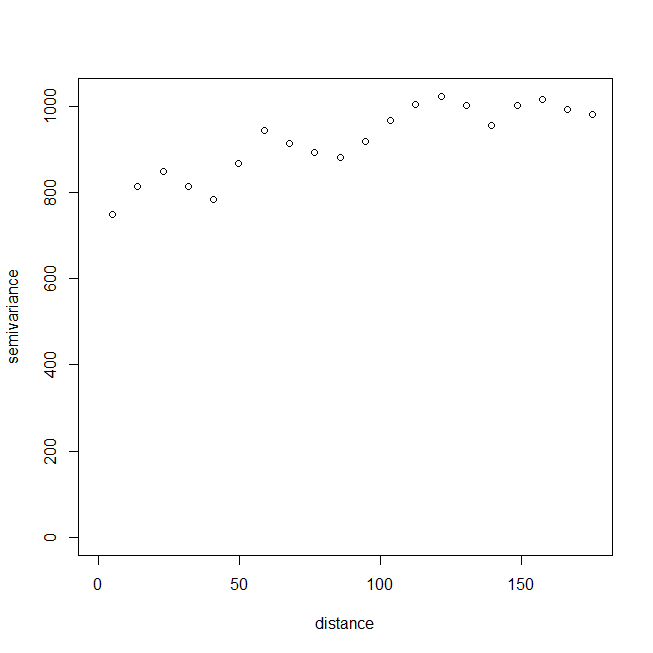
\includegraphics[scale=0.2,trim={2mm 5mm 2mm  5mm},clip]{../figures/wef_vario.png}}
	\subfloat[Residuals]{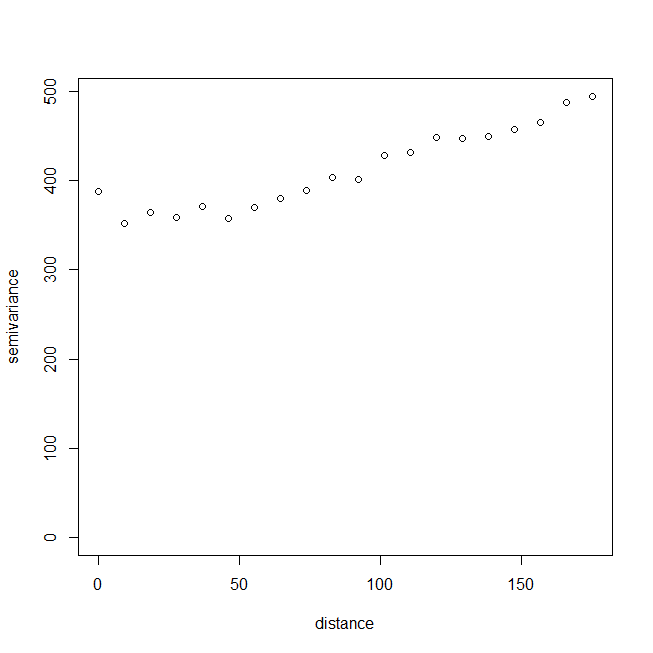
\includegraphics[scale=0.2,trim={2mm 5mm 2mm 5mm},clip]{../figures/wef_vario_res.png}}
\end{figure}
	\begin{itemize}
		\item Variogram of the residuals confirm \red{unexplained spatial variation}
	\end{itemize}
\end{frame}

%\section{Modeling spatial data with Gaussian Processes}

\begin{frame}{Modeling with the locations}
	\begin{itemize}
		\myitem When purely covariate based models does not suffice, one needs to leverage the information from locations
		\myitem General model using the locations: $y(s)=x(s)'\beta + w(s) + \eps(s)$ for all $s \in D$
		\myitem How to choose the function $w(\cdot)$?
		\myitem Since we want to predict at any location over the entire domain $D$, this choice will amount to choosing a \blue{surface} $w(s)$
		\myitem How to do this ? 
	\end{itemize}
\end{frame}

\begin{frame}{Gaussian Processes (GPs)}
	\begin{itemize}
		\item One popular approach to \blue{model} w(s) is via Gaussian Processes (GP)
		\item The collection of random variables $\{w(s) \given s\in D\}$ is a GP if 
		\begin{itemize}
			\item it is a \red{valid} stochastic process
			\item all finite dimensional densities $\{w(s_1),\ldots,w(s_n)\}$ follow multivariate Gaussian distribution
		\end{itemize}
		\item A GP is completely characterized by a mean function $m(s)$ and a covariance function $C(\cdot,\cdot)$
		\item \red{Advantage:} \blue{Likelihood} based inference. $w=(w(s_1),\ldots,w(s_n))' \sim N(m,C)$ where $m=(m(s_1),\ldots,m(s_n))'$ and $C=C(s_i,s_j)$
	\end{itemize}
\end{frame}

\begin{frame}{Valid covariance functions and isotropy}
	
	\begin{itemize}
		
		\item $C(\cdot,\cdot)$ needs to be \red{valid}.  For all $n$ and all $\{s_{1}, s_{2},..., s_{n}\}$, the resulting
		covariance matrix $C(s_i,s_j)$ for $(w(s_{1}), w(s_{2}),..., w(s_{n}))$ must be positive definite
		
		\item So, $C(\cdot,\cdot)$ needs to be a \blue{positive definite} function
		
		\item Simplifying assumptions: 
		\begin{itemize}
			\item \alert{Stationarity:} $C(s_1,s_2)$ only depends on $h = s_1 - s_2$ (and is denoted by $C(h)$)
			\item \alert{Isotropic:} $C(h) = C(||h||)$
			\item \alert{Anisotropic:} Stationary but not isotropic
		\end{itemize}
		
		\item Isotropic models are popular because of their \green{ simplicity, interpretability,} and because a number of relatively \green{ simple parametric forms} are available as candidates for $C$.
		
		%\item Much theory, characterization, construction, exemplification in the literature
		%
		%\item Why GPs are attractive - only need a mean function and a valid covariance function
	\end{itemize}
\end{frame}

%\begin{frame}{Isotropy}
%
%\begin{itemize}
% %\pause
%
%\item If the process is \green{ intrinsically stationary} with an \green{ isotropic} covariance function, it is also called \blue{ homogeneous}. %\pause
%
%\item Isotropic models are popular because of their \green{ simplicity, interpretability,} and because a number of relatively \green{ simple parametric forms} are available as candidates for $C$ (and $\gamma$). %Denoting $||h||$ by $t$ for notational simplicity, the next two tables provide a few examples.
%
%\end{itemize}
%\end{frame}
%
\begin{frame}{Some common isotropic covariance functions}
	\vspace{-0.25in}
	\begin{table}[t]
		\begin{center}
			\begin{tabular}{|ll|}\hline
				Model & Covariance function, $C(t)=C(||h||)$ \\\hline %
				Spherical & $C(t) = $ $\left \{ \begin{array}{cl}
				0 & \mbox{if } t\geq1/\phi\\
				\sigma^{2}\left[  1-\frac{3}{2}\phi t+\frac{1}{2}(\phi
				t)^{3}\right] &
				\mbox{if } 0<t\leq1/\phi\\
				\tau^{2}+\sigma^{2} &  \mbox{otherwise}
				\end{array} \right .$\\
				Exponential & $C(t) = $
				$\left \{ \begin{array}{cl}%
				\sigma^{2}\exp(-\phi t) & \mbox{if } t>0\\
				\tau^{2}+\sigma^{2} & \mbox{otherwise}\end{array} \right .$\\
				$\begin{array}{l}
				\!\!\! \mbox{Powered} \\
				\! \mbox{exponential}
				\end{array}$
				& $C(t) = $
				$\left \{ \begin{array}{cl}%
				\sigma^{2}\exp(-|\phi t|^{p}) & \mbox{if } t>0\\
				\tau^{2}+\sigma^{2} & \mbox{otherwise}
				\end{array} \right .$
				\\
				$\begin{array}{l}
				\!\!\! \mbox{Mat\'{e}rn}\\
				\! \mbox{at } \nu=3/2
				\end{array}$
				& $C(t) = $ $\left \{ \begin{array}{cl} \sigma^{2}\left(1+\phi
				t\right)  \exp({-\phi t}) &
				\mbox{if } t>0\\
				\tau^2 + \sigma^{2} &  \mbox{otherwise}
				\end{array} \right .$
				\\\hline
			\end{tabular}
			
		\end{center}
	\end{table}
\end{frame}

\begin{frame}{Notes on exponential model}
	
	$$
	C(t) = \left \{ \begin{array}{cl}
	\tau^2 + \sis &  \mbox{  if }t=0\\
	\sis \exp(-\phi t) &  \mbox{  if }t>0\\
	\end{array}\right . \; .
	$$%\pause
	
	\begin{itemize}
		
		\item We define the \alert{effective range},  
		$t_0$, as the distance at which this correlation has dropped to
		only 0.05. Setting $\exp(-\phi t_0)$ equal to this value we obtain
		$t_0 \approx 3/\phi$, since $\log(0.05) \approx -3$. %\pause
		
		\item The \alert{nugget} $\tau^2$ is often viewed as a \blue {``nonspatial effect variance,''}
		
		\item The  \alert{partial sill} ($\sigs$) is viewed as a \blue {``spatial effect variance.''} %\pause
		
		\item $\sigs + \taus$ gives the maximum total variance often referred to as the \alert{sill}
		
		\item Note \blue{discontinuity} at $0$ due to the nugget.  \red{Intentional!} To account for measurement error or micro-scale variability.
	\end{itemize}
\end{frame}


\begin{frame}{Covariance functions and semivariograms}
	\begin{itemize}
		\item \green{Recall:} Empirical semivariogram: $\gamma(t_k) = \frac{1}{2|N(t_k)|}\sum_{s_i,s_j \in
		N(t_k)}(Y(s_i)-Y(s_j))^2$ 
	\item For any stationary GP, $E(Y(s+h)-Y(s))^2/2 = C(0)-C(h) = \gamma(h)$
	\item $\gamma(h)$ is the \alert{semivariogram} corresponding to the covariance function $C(h)$
	\item \green{Example:} For exponential GP, $\gamma(t) = 
	\left \{ \begin{array} {cl}%
	\tau^{2}+\sigma^{2}(1-\exp(-\phi t)) & \mbox{if } t>0\\
	0 & \mbox{if } t=0
	\end{array} \right .$, where $t=||h||$
	\end{itemize}
\end{frame}

\begin{frame}{Covariance functions and semivariograms}
	\begin{figure}
		\only<1>{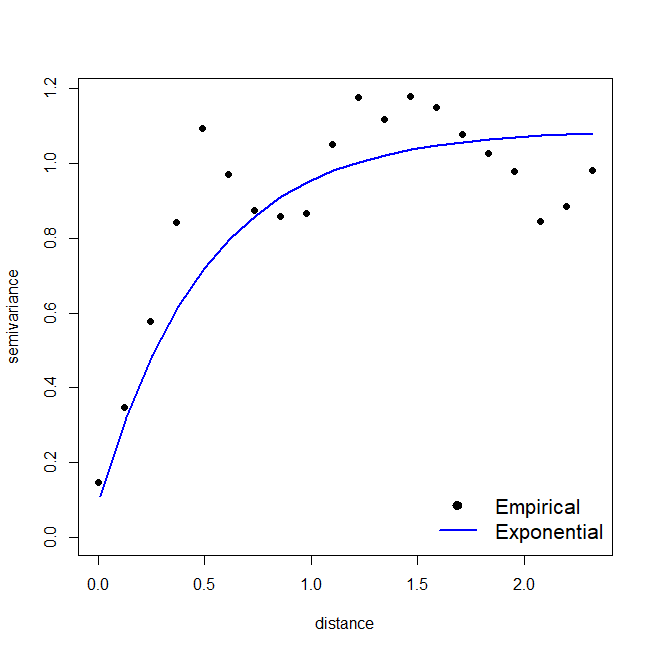
\includegraphics[scale=0.25]{../figures/exp_vario.png}}
		\only<2>{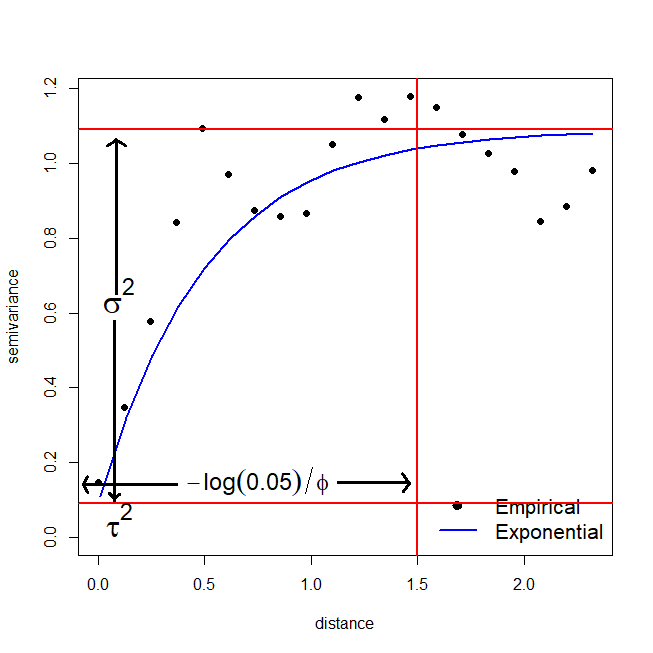
\includegraphics[scale=0.35]{../figures/exp_vario2.png}}
	\end{figure}
\end{frame}


\begin{frame}{The Mat\`{e}rn covariance function}
	
	\begin{itemize}
		%\item Much of statistical modeling is carried out through
		%correlation functions rather than variograms %\pause
		
		\item The Mat\`{e}rn is a very versatile family:
		\[
		C(t) = \left\{
		\begin{array}{cc}
		\frac{\sigma^2}{2^{\nu-1}\Gamma(\nu)} (2\sqrt{\nu}t\phi)^{\nu}K_{\nu}(2\sqrt(\nu)t\phi) & \text{if } t > 0 \\
		\tau^2 + \sigma^2 & \text{if } t=0\\
		\end{array}
		\right.
		\]
		$K_{\nu}$ is the modified Bessel function of order $\nu$
		(computationally tractable) %\pause
		
		\item $\nu$ is a smoothness parameter %(a \emph{fractal}) 
		controlling process smoothness.  \blue{Remarkable!}
		
		\item $\nu=1/2$ gives the exponential covariance function
	\end{itemize}
\end{frame}

\begin{frame}{Kriging: Spatial prediction at new locations}
	\begin{itemize}
		\item \red{Goal:} Given observations $w=(w(s_1), w(s_2), \ldots, w(s_n))'$, predict $w(s_0)$ for a new location $s_0$
		\item If $w(s)$ is modeled as a GP, then $(\red{w(s_0)}, w(s_1), \ldots, w(s_n))'$ jointly follow multivariate normal distribution
		\item $w(s_0) \given w$ follows a normal distribution with
			\begin{itemize}
				\item Mean (\alert{kriging estimator}): $m(s_0) + c'C^{-1}(w-m)$ 
				\item where $m=E(w)$, $C=Cov(w)$, $c=Cov(w,w(s_0))$
				\item Variance: $C(s_0,s_0) - c'C^{-1}c$
			\end{itemize}
		\item The GP formulation gives the \blue{full predictive distribution} of $w(s_0) | w$ 
	\end{itemize}
	\end{frame}

\begin{frame}{Modeling with GPs}
	\metroset{block=fill}{
	\begin{alertblock}{Spatial linear model}
		\[y(s)=x(s)'\beta + w(s) + \eps(s)\]
	\end{alertblock}}
	\begin{itemize}
		\item $w(s)$ modeled as $GP(0,C(\cdot\given \theta))$ (usually without a nugget)
		\item $\eps(s) \iid N(0,\taus)$ contributes to the nugget
		\item Under isotropy: $C(s+h,s) = \sigs R(||h|| \; ; \phi )$
		\item $w = (w(s_1),\ldots,w(s_n))' \sim N(0, \sigs R(\phi))$ where $R(\phi) = \sigs (R(||s_i-s_j|| \; ; \phi))$
		\item $y=(y(s_1),\ldots,y(s_n))' \sim N(X\beta,\sigs R(\phi) + \taus I)$
		%\item Kriging: $y(s_0) \given Y \sim N(x'\beta + c_0'(\sigs R(\phi) + \taus I)^{-1}(Y-X\beta), \sigs+\taus - c_0'(\sigs R(\phi) + \taus I)^{-1}c_0)$
	\end{itemize}
\end{frame}

\begin{frame}{Parameter estimation}
\begin{itemize}
	\item $y=(y(s_1),\ldots,y(s_n))' \sim N(X\beta,\sigs R(\phi) + \taus I)$
	\item We can obtain MLEs of parameters $\beta, \taus, \sigs, \phi$ based on the above model and use the estimates to krige at new locations
	\item In practice, the likelihood is often very \red{flat} with respect to the spatial covariance parameters and choice of \blue{initial values} is important
	\item Initial values can be eyeballed from empirical semivariogram of the residuals from ordinary linear regression
	\item Estimated parameter values can be used for kriging
\end{itemize}
\end{frame}

\begin{frame}{Model comparison}
	\begin{itemize}
		\item For $k$ total parameters and sample size $n$:
		\begin{itemize}
			\item \alert{AIC:} $2k - 2 \log (l(y \given \hat\beta, \hat\theta, \hat\taus))$
			\item \alert{BIC:} $\log(n) k - 2 \log (l(y \given \hat\beta, \hat\theta, \hat\taus))$
		\end{itemize}
		\myitem Prediction based approaches using holdout data:
		\begin{itemize}
			\item Root Mean Square Predictive Error (\alert{RMSPE}): $\sqrt{\frac 1{n_{out}}\sum_{i=1}^{n_{out}} (y_i - \hat y_i)^2}$
			\myitem Coverage probability (\alert{CP}): $\frac 1{n_{out}} \sum_{i=1}^{n_{out}} I(y_i \in (\hat y_{i,0.025}, \hat y_{i,0.975}))$
			\myitem Width of $95\%$ confidence interval (\alert{CIW}): $\frac 1{n_{out}} \sum_{i=1}^{n_{out}} (\hat y_{i,0.975}- \hat y_{i,0.025})$
			\myitem The last two approaches compares the distribution of $y_i$ instead of comparing just their point predictions
		\end{itemize}
	\end{itemize}
\end{frame}

\begin{frame}{Back to WEF data}
		\begin{table}
			\caption{Model comparison}
			\begin{tabular}{@{} ccc @{}}
				\toprule
				& Spatial & Non-spatial\\
				\midrule
				AIC & 4419 & 4465\\
				BIC & 4448 & 4486\\
				\midrule
				RMSPE & 18 & 21\\
				CP & 93 & 93\\
				CIW & 77 & 82\\
				\bottomrule
			\end{tabular}
		\end{table}
\end{frame}	

\begin{frame}{WEF data: Kriged surfaces}
	\begin{figure} 
		\begin{center}
			\hskip -1mm \subfloat[DBH Estimates]{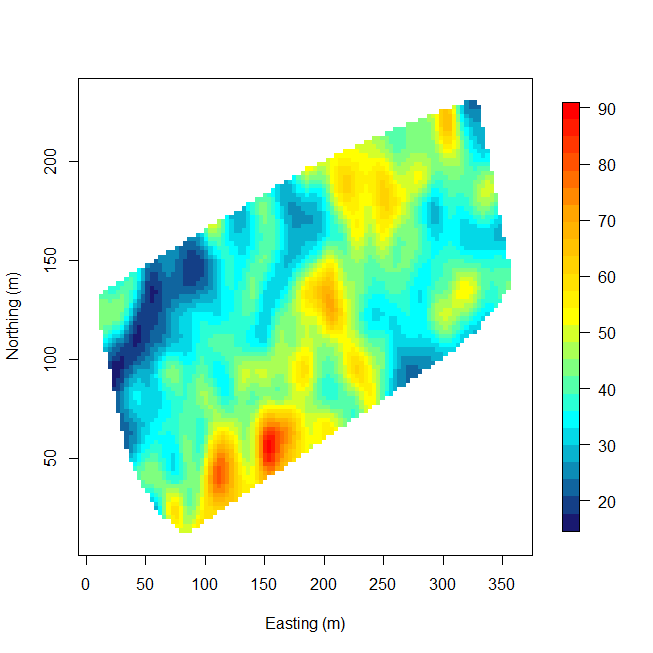
\includegraphics[scale=0.15]{../figures/wef_pred.png}}
			\subfloat[Standard errors]{ 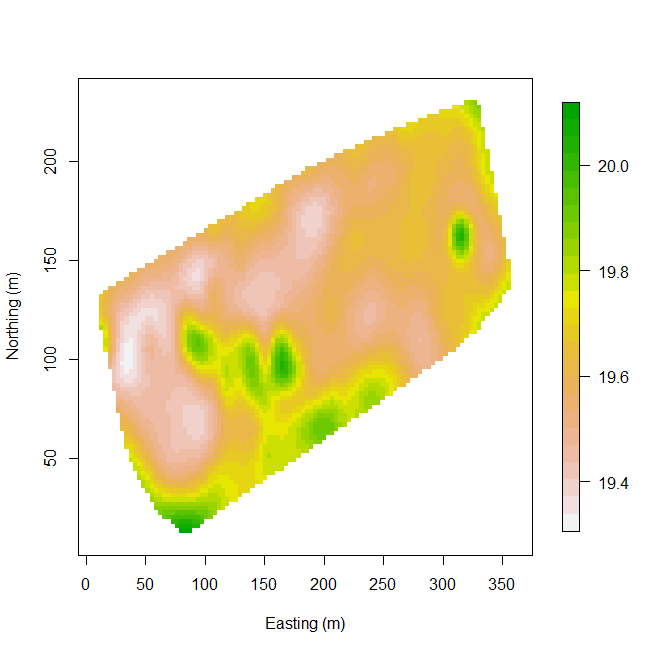
\includegraphics[scale=0.15]{../figures/wef_predsd.png}}
		\end{center}
	\end{figure}
\end{frame}

%\begin{frame}[standout]
%  Questions?
%\end{frame}

\begin{frame}{Summary}
\begin{itemize}
\item Geostatistics -- Analysis of point-referenced spatial data
\item Surface plots of data and residuals
\item EDA with empirical semivariograms
\item Modeling unknown surfaces with Gaussian Processes
\item Kriging: Predictions at new locations
\item Spatial linear regression using Gaussian Processes
\end{itemize}
\end{frame}

\end{document}
